\chapter{Overview of the experiment and testing environment}
\label{chp:problem}
The data for the project was extrapolated from a testing campaign to analyze the behavior of the
High Order corrector superconducting magnets. These magnets have been designed to produce five
different multipolar field orders (quadrupole, sextupole, octapole, decapole, and dodecapole) to
correct the magnetic field irregularities introduced by the focusing quadrupoles; which reduce the
cross-section of the two counter-rotating protonic beams in the proximity of interaction regions
(sections of the LHC ring in which the particles encounter during high-energy experiments). Such
irregularities need correction since they might lead to:
\begin{inparaenum}[(i)]
	\item instability,
	\item beam degradation,
	\item increase in the emittance of the beam, which is the area occupied by the beam in the
	position--momentum space.
\end{inparaenum}

The original work~\cite{mariotto2022}, consisted in a test campaign in which the HO correctos
marngets, kept at cryogenic temperature at the \textsc{infn} Laboratorio Acceleratori e Superconduttività
Applicata in Milan, were powered to evaluate their performances and thermal stability up to the
nominal operating condition. During magnet powering, spontaneous transitions to the
normal-conducting state can occur due to mechanical instability of the winding or stress induced by
the Lorentz forces acting on the conductors. Each magnet is protected using a classical resistive
voltage detection system and discharged on an external dumping resistance to extract the magnetic
energy and prevent material damage. Since different classes of magnets were tested we chose to use
two voltage taps to collect the voltage data, this means that the quench detection system can only
localize quench developing in one half of the magnet or the other, without the possibility of
localizing precisely which superconducting winding started the transition to the normal conducting
state\todo{Capire perché non si sono usati più voltage taps diversi}.\begin{figure}[h!]
	\centering
	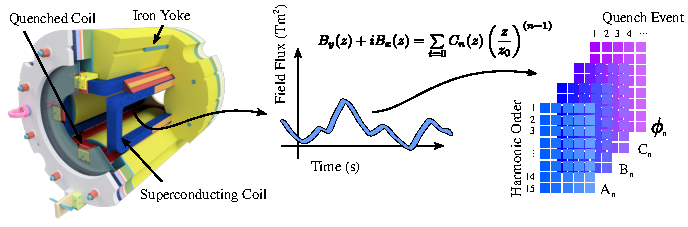
\includegraphics[width=\linewidth]{img/FieldProcedure.pdf}
	\caption{Sketch of the magnetic field measurements after a quench event for the quadrupole magnet and dataset obtained for each quench event measurement.}
	\label{fig:FieldMeasurement}
\end{figure}
In the original work the condition of a superconducting coil was recognized based on the analysis of
the residual magnetic field. If the magnet was in working order, the residual magnetic field was
expected to be $\neq 0$. If one of the coils in the magnet assembly quenched, all the energy therein
contained would have been dumped on the resistance (due to the Quench Protection System activation),
therefore its residual magnetic field would be $\approx 0$, leading to an unexpected geometry of the
superposition of the coil contributions.\todo{Non so se ho scritto delle cazzate -- Bigi} Since the
quadrupoles, magnets MQSXF1 to MQSXF6, registered the majority of the quench events, due to their
high operating current, the original work focused on them and our work follows the same logic. The
results of the test campaign were $279$ different measurements only on quadrupoles, including those
identifying the magnet in good working condition, and quenches.

Harmonic decomposition of magnetic field, or multipolar expansion, is a classic technique used to
analyze magnetic field quality and is detailed in~\cite{ambrosio1996-mexpansion}. If we consider a
$2$D approximation of the magnet on the $X-Y$ plane, a point $z_0$ in the $X-Y$ plane and a current
$I$ flowing along the third axis $z$; the magnetic field $B(z_0)$ can be expressed as
\begin{equation}
	\label{eq:bz}
	|B(z_0)| = \frac{\mu_0I}{2\pi d}
\end{equation}
where $d$ is the distance between our point $z_0$ and the $z$ axis. The magnetic field can be
expressed as a complex number
\begin{equation}
	\label{eq:bcomplex}
	\begin{aligned}
		 & B_z = 0 \enspace,         \\
		 & B  = B_x + iB_y \enspace.
	\end{aligned}
\end{equation}
Since we can express $z_0$ as a point in complex bidimensional space: $z_0 = x_0 + iy_0$, we can
rewrite~\ref{eq:bz} as the product of the modulus $|B(z_0)|$ and the versor normal to the segment $\overline{zz_0}$:
\begin{equation}
	\label{eq:bzcomplex}
	\begin{aligned}
		B & = B_x + iB_y                                              \\
		  & = \frac{mu_0I}{2\pi|z_0 - z|}\frac{i(z_0 - z)}{|z_0 - z|} \\
		  & = \frac{mu_0I}{2\pi}\frac{i}{z_0^* - z^*} \enspace.
	\end{aligned}
\end{equation}
Where $z^*$ and $z_0^*$ are, respectively, the conjugates of $z$ and $z_0$. Instead of using $B$ we
compute the value of the complex conjugate $B^*$
\begin{equation}
	\label{eq:bconj}
	\begin{aligned}
		 & B^* = B_x - iB_y = \frac{\mu_0I}{2\pi}\frac{i}{z - z_0}                     \\
		 & \text{since} \hspace{10pt} \left(\frac{i}{a + ib}\right)^* = \frac{i}{-(a +
			ib)^*} \enspace.
	\end{aligned}
\end{equation}
This because the conjugate is an analytic function\footnote{
	An analytic function is a function that is locally given by a convergent power series. In
	general, a function is analytic if it respects the Cauchy Theorem which is stating that: Let
	$D$ be a finite, simply connected domain and $C$ any closed, rectifiable curve contained in
	$D$. If the function $f(z)$ is differentiable in the domain $D$, then the integral of $f(z)$
	along $C$ is equal to $0$. Which means that the function is analytic~\cite{evgrafov2019analytic}.
} which makes it more useful for two reasons:
\begin{itemize}
	\item We can expand it in power series, leading us to multipolar expansion,
	\item for a given region, the maximum value of the modulus is on the boundary. This is
	      identifies the maximum field point within the magnet (even though $B^*$ is not
	      analytic within the magnet we can use equivalent functions for it).
\end{itemize}
Since~\ref{eq:bconj} is analytic then we can do a power series expansion on $z$, and we can rewrite:
\begin{equation}
	\label{eq:pexp}
	\frac{1}{z - z_0} = \frac{1}{z} \sum_{n = 1}^\infty \left(\frac{z_0}{z}\right)^n = \sum_{n =
		1}^\infty \frac{z_0^{n - 1}}{z^n} \enspace.
\end{equation}
We can rewrite~\ref{eq:bconj} for a uniformly distributed current density $J$ on an arbitrary
cross-section $\sigma$ as
\begin{equation}
	\label{eq:bconj-generic}
	B^* = i \frac{\mu_0J}{2\pi}\int_{\sigma}\frac{1}{z - z_0}da \enspace.
\end{equation}
If we apply the power-series expansion to the equation we just found:
\begin{equation}
	\begin{aligned}
		 & B^*(z_0) = \sum_{n = 1}^\infty C_n z_0^{n - 1} \enspace,                        \\
		 & \text{with}\hspace{10pt}C_n = i \frac{\mu_0J}{2\pi}\int_{\sigma}\frac{1}{z^n}da
		\enspace .
	\end{aligned}
\end{equation}
The $C_n$ are non-normalized multipolar coefficients:
\begin{itemize}
	\item $C_1$ is the \emph{dipolar} field harmonic,
	\item $C_2$ is the \emph{quadrupolar} field harmonic,
	\item $C_3$ is the \emph{sestupolar} field harmonic;
\end{itemize}
and so on and so forth. These multipolar coefficients highlight the fact that any magnet generating
a certain magnetic field (e.g., a quadrupolar magnet generates quadrupolar field), contians
multipolar harmonics that disturb the main component. In the context of our example, a quadrupolar
magnetic field generates a main quadrupolar component but introduces sestupolar, ottupolar, \ldots
harmonics that disturb the main field.

Since the multipolar coefficient is a complex number it can be expressed as $C_n = A_n - iB_n$, the components
\begin{inparaenum}[(i)]
	\item $A_n$s generate the horizontal fields and are known as \emph{skew} components,
	\item $B_n$s enerate the vertical fields and are called \emph{right} components.
\end{inparaenum}

For each event, 60 samples of harmonic coefficients have been measured and averaged to obtain a single set of $15$ different magnetic field harmonics coefficients which contain all the information of the produced magnetic field quality (see Fig.~\ref{fig:FieldMeasurement}). Recalling that these coefficients are expressed as complex numbers, the information have been organized in terms of the following four attributes, in which the suffix $n \in \{1, \dots,  15\}$ is related to a specific harmonic:
\begin{itemize}
	\item the imaginary part \an, of the $n^\text{th}$ field harmonic coefficient;
	\item the real part \bn, of the $n^\text{th}$ field harmonic coefficient;
	\item the absolute value \cnmod, of the $n^\text{th}$ field harmonic coefficient;
	\item the phase \phin, of the $n^\text{th}$ field harmonic coefficient.
\end{itemize}
Since the magnets in the original testing campaign were mounted skewed: the $A_n$
feature was supposed to be highly informative since they are directly correlated with the rotational
position of the quenched coil in the magnet assembly. The absolute values $|C_n|$ would be a
valuable feature for \qrp{} and not for \qlp{} since two different configurations with the same
number of quenched coils but different angular positions would give the same harmonic content and
different phases.\todo{Riguardare con Samuele questa parte riguardo a Cnmod -- Bigi} Each measurement was coupled with a \emph{label} encoded as follows:
\begin{itemize}
	\item a simple binary flag for \qrp, where $1$ means that a quench has happened, while $0$ characterizes the normal working conditions of the superconductor;
	\item four binary flags for \qlp, each describing a  coil and stating whether or not a quench happened within it, using the same encoding as in previous point.
\end{itemize}
We remark here that the labels for \qrp\ were reasonably balanced: namely, the number of non-quench events was of $87$ while the number of quench events was of $192$; concerning \qlp, on the other hand, every coil has a different distribution: as detailed in Table~\ref{tab:balance}, the proportion of quench over non-quench events roughly ranges from $30\%$ to $50\%$. It is important to notice that the sum of all quench events for \qlp\ is not $192$, since one quench event for \qrp\ could have been caused by up to three different coils (e.g., coils 0, 1 and 3) quenching at the same time.

\begin{table}[h]
	\caption{Label distribution for the various coils in \qlp.}\label{tab:balance}

	\bigskip
	\setlength{\tabcolsep}{6pt}
	\centering
	\begin{tabular}{ccc}
		\toprule
		\textbf{Coil} & \textbf{Quench} & \textbf{Non-quench} \\
		\midrule
		0             & 68              & 211                 \\
		1             & 96              & 183                 \\
		2             & 79              & 200                 \\
		3             & 73              & 206                 \\
		\bottomrule
	\end{tabular}
\end{table}

In each of our experiments we did not use all attributes, in most cases the datasets aggregated the
best harmonics for a certain attribute (e.g., \an[2] and \an[12]). We will refer to these as sub-views of an attribute.

The objective of the thesis was to find machine learning models capable of:
\begin{enumerate}
	\item recognizing whether the magnet underwent a quench event during operation, which we will refer
	      to as Quench Recognition Problem (\qrp) from now on, and will be treated in \Cref{chp:qrp};
	\item recognize, if the superconductor quenched, which coil(s) transitioned; we will refer to
	      it as Quench Localization Problem (\qlp) from now on, and it will be treated in
	      \Cref{chp:qlp}.
\end{enumerate}
The models chosen to solve \qrp\ and \qlp\ had to be both reliable and highly explainable to favour
further study of quench phenomenon on High-Order corrector magnets.

\section{Model selection and model testing procedures}
Reproducibility is a key property of any experiment, to cover the basics, we set the seed for all
random number generators to the same value, and we used shared pipelines for all our experiments.

Sub-views are built using a common pipeline that generates three different datasets, serialized
for later reuse, an overview of the datasets is given here below.
\begin{itemize}
	\item The \emph{merged} dataset, \dm, which constructs a single table out of all the
	      measurements done on the attribute(s) for the different magnets. Before serialization, the
	      data is standardized.
	\item The \emph{blind-test} dataset, \db, contains a small part of the overall data available to us
	      ($29$ samples), these samples were kept locked until the experiments were considered
	      complete. Using the blind-test set we performed a final test on the best models to see
	      how well the performance generalized on unseen data.
	\item The \emph{reduced} dataset, \dr, contains the rest of the samples, $250$ in total,
	      and is the main set used to perform experiments.
\end{itemize}

Model selection and testing were carried out using Nested Cross Validation (\ncv). \ncv\ is suitable
for situations in which the data is not abundant~\cite{Larracy2021} due to its heavy reuse, enabling
model selection and testing; while also giving less biased performance estimates by averaging the
results on $k$ different folds. In the following section we will do a rapid excursus on how the
cross-validation procedure works.

\subsubsection{Cross Validation}
\label{sec:cv}
In \Cref{chp:ml} we outlined the simple train-test splitting procedure, now we will introduce an
alternative technique that gives us a powerful tool to prevent overfitting and get less biased performance measures while also doing hyperparameter selection.

$k$-fold \cv~\cite{ZhouZhi-Hua2021ML} is a splitting technique that divides a dataset $D$ in $k$
different folds $\fold{i}, i \in \{1, \ldots, k\}$; the folds are non-overlapping and about the same
size, therefore
\[\fold{i} \cap \fold{j} = \emptyset \hspace{5pt} \forall i, j \in \{1, \ldots, k\}, i \neq j \enspace,\]
and the union of all the folds is the original dataset
\[\bigcup_{i \in \{1, \ldots, k\}} \fold{i} = D \enspace.\]

In the framework of train-test splitting, if we used the procedure outlined in \Cref{sec:sml}, we
would split the original dataset into the training set $T$ and the generalization set $G$, train a
model $\model$ on $T$ and then test the performance on $G$. While this is a perfectly acceptable procedure
to gather performance metrics for a model, it gives us reliable performance metrics only if the
dataset contains many samples. The bigger the dataset $D$ the more samples can go in both $T$ and
$G$ making sure that many different cases are covered.

By measuring performance on different folds (each one is a self-contained train-test procedure), we
get a more complete vision of the model performance: each sample in the dataset has been used
\emph{at least once} for training and \emph{one single time} for testing. The fold structure allows
us to recognize pathological situations, like cases in which the standard deviation of the fold
performance is very wide. To understand how the folds are constructed, let's consider an example in which $5$-fold \cv\ is computed on a dataset containing $250$ samples: $5$ different models are generated, each time trained on $200$ samples and then tested on the remaining $50$ samples (the testing fold changes with every iteration).

\smallskip

The number of folds to be used for \cv\ becomes another hyperparameter of the problem, since it
depends on many factors like the amount of available data or the required reliability of performance
reads. A large value of $k$ will increase the number of folds the model is trained and tested on,
increasing the robustness of the performance estimation at the expense of computational complexity
(e.g., Leave One Out \cv\ is an example of such approaches, in~\cite{shao2016} a more efficient
approach to the technique is discussed); too small a value of $k$ makes the \cv\ less robust but more efficient (classic values of $k$ for most practical uses are $5, 10, 20$).

\smallskip

Let us now move to a more complicated environment in which we need, given a base model, to fine tune
it, train it and test it. We can na\"ively tripartition dataset $D$:
\begin{itemize}
	\item \emph{training set} $T$, which is the same set we defined in \Cref{sec:sml} but is now
	      used to fine tune the hyperparameters of the model,
	\item \emph{validation set} $V$, this set of samples will be used to test the performance of the
	      model found after the training step,
	\item \emph{generalization set} $G$, after the model is retrained on $T \cup V$ the performance are
	      tested on $G$ to see if the model is capable of generalizing effectively.
\end{itemize}

Once again we cannot guarantee that:
\begin{inparaenum}[(i)]
	\item the chosen model is the best one,
	\item the performance metrics obtained from the single generalization fold are actually reliable.
\end{inparaenum}
To address the issue we can substitute each procedure with $k$-fold \cv, one nested inside the other
one, the \emph{inner} is used to do model selection, the \emph{outer} is used to test performance
for the model just generated. To get a better understanding of the Nested cross-validation procedure
(\ncv) just introduced, let us consider a $5 \times 5$ \ncv\ procedure applied to a dataset of $250$
samples (an outline of the \ncv\ procedure is shown in \Cref{fig:nested-cv}).
\begin{enumerate}
	\item The data is first split into $5$ folds of $50$ samples. One fold of $50$ samples will
	      be kept on the side for the generalization test, the remaining $200$ samples will be used to do both training and model selection;
	\item The training set is now split again in $5$ folds, $160$ samples will be used to do
	      model selection, $40$ samples will be used to validate the performance that has been
	      found. In practice, as was anticipated in \Cref{sec:sml}, when we do model selection
	      (or hyperparameter fine-tuning) we explore only a very limited portion of the
	      hyperparameter space to find the combination that in yields the best performance
	      during validation. \emph{De facto}, we used a hyperparameter grid (cfr. \Cref{tbl:params}), for all the
	      possible combinations we trained a model and validated its performance
	\item Step 2 until all folds have been used for validation (therefore every sample in
	      the training set has been used once to test the performance of the model).
	\item The model found at the previous step is retrained on the whole $200$ training samples, then the performance is tested on the fold that was kept aside in the first step.
	\item Steps 1, 2, 3, 4 are repeated until every sample in the original dataset has been used
	      only one time for the final testing run.
\end{enumerate}
\todo{Rivedere la sezione sulla Cross validation perché è abbastanza astrusa -- Ale}
\begin{figure}[!t]
	\centering
	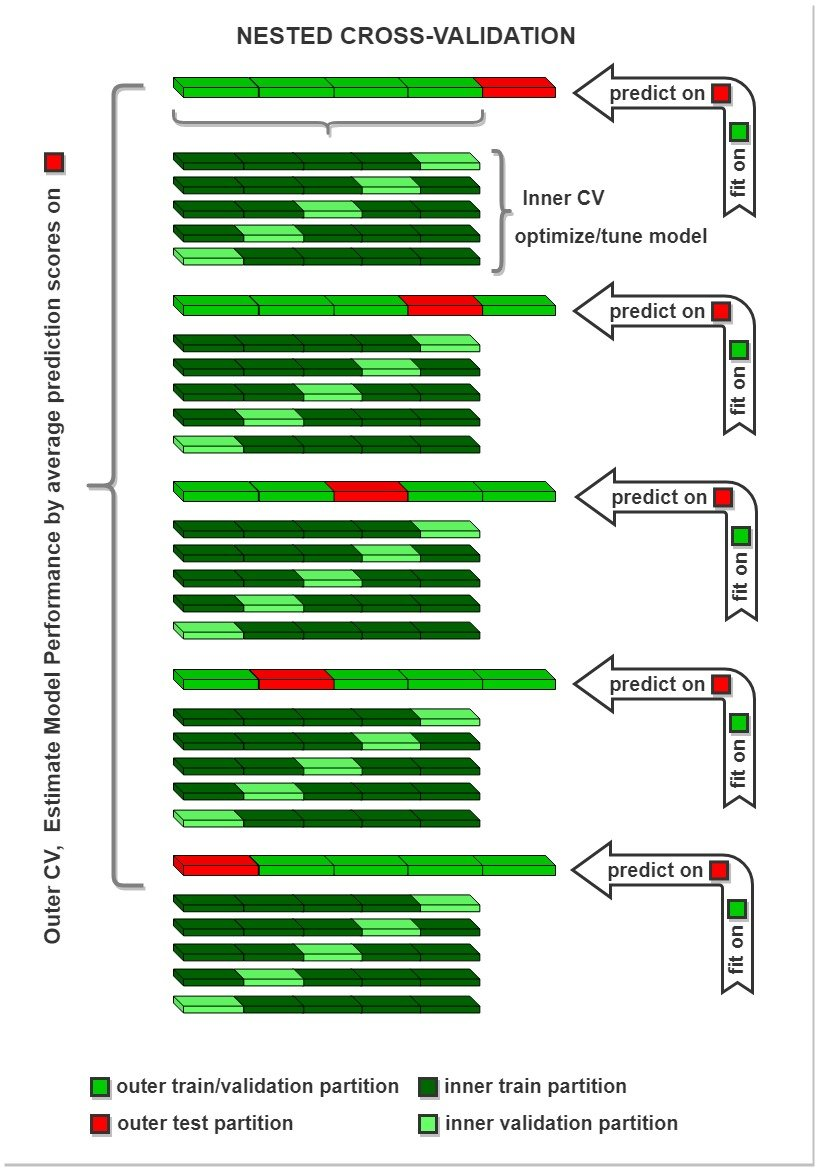
\includegraphics[scale=.3]{./img/nested-cv.png}
	\caption{Visualization of the nested cross validation procedure taken from~\cite{lavasa2021}}
	\label{fig:nested-cv}
\end{figure}

Once the \ncv\ procedure terminates we will get $k$ different models, since the fine-tuned models
are statistically equivalent, thus we can decide the one to keep based on the heuristic that fits our
objectives the best.

The closing section for this chapter will contain a summarization of the experimental setup.

\section{Experimental setup}
All experiments have been executed using Python 3.10.12 (the latest version at the time of writing), using the following libraries: scikit-learn (release 1.5.2) for data preprocessing and model training and evaluation, numpy (release 2.2.3) for efficient data storage, and Pandas (release 2.2.3) for data management. These libraries have been handled through the pip package manager (release 25.0.1) and used within a virtual environment.

The seeds from the various random number generators have been set to the common value of
\href{https://www.google.com/search?q=the+answer+to+life+the+universe+and+everything&num=10&client=firefox-b-d&sca_esv=a81abf9bb67ffd9b&sxsrf=AHTn8zo6RKep_zuEvIhJb5nuAGh5xAERLg\%3A1739739141586&ei=BVCyZ_C9I9mLi-gP7e-B8Ac&oq=the+answer+to+&gs_lp=Egxnd3Mtd2l6LXNlcnAiDnRoZSBhbnN3ZXIgdG8gKgIIADIIEAAYgAQYywEyCBAAGIAEGMsBMgUQABiABDIIEAAYgAQYywEyCBAAGIAEGMsBMggQABiABBjLATIIEAAYgAQYywEyCBAAGIAEGMsBMggQABiABBjLATIIEAAYgAQYywFIjCJQqQlYiRlwA3gBkAEAmAFuoAHICaoBBDExLjO4AQPIAQD4AQGYAhGgAv0JwgIKEAAYsAMY1gQYR8ICChAjGIAEGCcYigXCAgsQABiABBixAxiDAcICCxAuGIAEGLEDGIMBwgIOEC4YgAQYsQMY0QMYxwHCAg4QLhiABBixAxiDARiKBcICERAuGIAEGLEDGNEDGIMBGMcBwgIMECMYgAQYExgnGIoFwgIEECMYJ8ICDRAuGIAEGEMY1AIYigXCAgoQABiABBhDGIoFwgIOEC4YgAQYxwEYjgUYrwHCAgoQLhiABBhDGIoFwgIIEC4YgAQYsQPCAggQABiABBixA8ICCxAuGIAEGLEDGNQCwgIFEC4YgATCAggQLhiABBjLAcICCxAuGIAEGNEDGMcBmAMAiAYBkAYIkgcEMTIuNaAHrboC&sclient=gws-wiz-serp}{42}
ensure replicability of the experiments.

The original dataset contained $279$ samples: for \qrp, each sample consisted of $15$ harmonics and
a label, stating whether the sample represents a quench event ($1$) or not ($0$); while for \qlp each sample had $4$ different
labels associated to it representing whether each one of the coils ($0$ for East, then: North, West and
South) quenched ($1$) or not ($0$).

Every splitting operation was performed by stratifying on the labels, in the case of \qlp, if the
labels were more than one, we used a multi-class stratification technique, detailed in~\cite{skmlearn}.

Experiments were conducted on three different computers running different architectures and
different operating systems, but the results did not change due to the standard-oriented approach.
See \Cref{tbl:computers} for a summary of the computers we used.
\begin{table}[t]
	\caption{System configuration used for our experiments. Core count values are detailed as number
		of CPU cores and threads, while frequency is expressed in the base and boost specifications.
		Finally, the CPU cache size is shown for the L1, L2 and L3 levels, where
		available.}\label{tbl:computers}

	\bigskip

	\centering
	\setlength{\tabcolsep}{4pt}
	\begin{tabular}{lccc}
		\toprule
		                     & \textbf{Pigna}        & \textbf{Mattone}         & \textbf{Topone}    \\
		\midrule
		\textbf{Model}       & Macbook Pro           & Custom build             & Dell XPS 8700      \\
		\textbf{CPU}         & i$5$ $5287\textsc{u}$ & Ryzen 7 $3700\textsc{x}$ & i$7$ $4770$        \\
		\textbf{Core count}  & $2\cc / 2\tds$        & $8\cc / 16\tds$          & $4\cc /
		8\tds$                                                                                       \\
		\textbf{Launch Date} & Q$1$ 2015             & Q$2$ 2019                & Q$2$ 2013          \\
		\textbf{Frequency}   & $2.90 / 3.30$ \ghz    & $4.125 / 4.40$ \ghz      & $3.40 / 3.90$ \ghz \\
		\textbf{Cache}       & $3$ \mb               & $0.512 / 4 / 32$ \mb     & $8$ \mb            \\
		\textbf{TDP}         & $28$ \w               & $84$ \w                  & $65$ \w            \\
		\textbf{RAM}         & $8$ \gb               & $16$ \gb                 & $16$ \gb           \\
		\textbf{OS}          & Pop!\_OS $22.04$ LTS  & Pop!\_OS $22.04$ LTS     & Fedora $39$        \\
		\bottomrule
	\end{tabular}
\end{table}
Experiments were dispatched on different systems based on the expected computational load.

Model selection was handled by doing a partial exploration of the parameter space (as mentioned in
\Cref{sec:cv}) via a grid search algorithm (GridSearchCV in scikit-learn), in which each model we defined a custom parameter grid (shown in \Cref{tbl:params}).

\begin{table}[t]
	\caption{Hyperparameters which we have tuned during the model training phase.} \label{tbl:params}

	\bigskip

	\centering
	\setlength{\tabcolsep}{6pt}
	\begin{tabular}{llc}
		\toprule
		\textbf{Model}       & \textbf{Hyperparameter}                                           & \textbf{Values}                        \\
		\midrule
		\multirow{5}{*}{DT}  & impurity criterion                                                & gini, entropy, log loss                \\
		                     & max depth                                                         & $2, 3, 4, 5$                           \\
		                     & min impurity decrease                                             & $0.001, 0.01, 0.05$                    \\
		                     & max features                                                      & None, $0.5, 0.75$                      \\
		                     & min samples leaf                                                  & $5, 10, 20$                            \\
		\midrule
		\multirow{2}{*}{RF}  & n. of trees                                                       & $2, 3, 5, 10$                          \\
		                     & \multicolumn{2}{l}{$+$ the same hyperparameters and values of DT}                                          \\
		\midrule
		\multirow{5}{*}{SVC} & $C$                                                               & $0.1, 1, 10, 100, 1000$                \\
		                     & $\gamma$                                                          & scale, auto, $0.001, 0.01, 0.1, 1, 10$ \\
		                     & degree                                                            & $2, 3, 4, 5$                           \\
		                     & $c_0$                                                             & $0, 0.1, 0.5, 1$                       \\
		                     & kernel                                                            & linear, poly sigmoid, rbf              \\
		\bottomrule
	\end{tabular}
\end{table}

All models have been tested on a suite of scorers meant to give us a more complete
understanding of how well the model is performing. The metrics are explained here below and, as
usual, by positive (negative) sample we mean a sample having label $1$ ($0$), and by true (false)
positive we mean a correctly classified positive (negative) sample:
\begin{itemize}
	\item \emph{Accuracy} (Acc): fraction of correct predictions,
	\item \emph{Precision} (Prc): number of true positives over number of positive predictions,
	\item \emph{Recall} (Rec): number of true positives over number of positive items,
	\item \emph{F1 score} (F1): harmonic mean between Precision and Recall,
	\item \emph{Inverse recall} (Irec): number of true negatives over number of negative items,
	\item \emph{ROC AUC} (RAUC): area under the ROC curve, the higher the value the further the
	      model is from being a random classifier.
\end{itemize}
Among all metrics we chose accuracy as the one leading model selection and main scorer since it
gives us a rough idea of the model performance: a high accuracy means that the model is
capable of recognizing well both positives and negatives. While this metric alone cannot tell us the
whole story (for instance, with a very high accuracy that is only sending $1$ as output), is a very
good large-grain metric. Any finer analysis can be done using the other metrics just described.





